
\subsection{Alimentación}
Se eligió utilizar una fuente partida de $\pm$60V  debido a que se buscaba una tensión de salida elevada para obtener un valor de potencia sobre la carga de $\approx 1KW$, para esto la tensión en modo diferencial debe ser de $\approx$ 90V, defininedo asi la tensión de alimentación.\\
También se optó por utilizar un segundo riel de alimentación para el par diferencial, teniendo como objetivo optimizar el rendimiento, dado que este trabaja con pequeña señal. Se optó por un valor de $\pm$ 15V, utilizando una resisitencia y un diodo zener para proveer esa tensión a partir de la fuente partida principal.
\begin{figure}[H]
\centering
	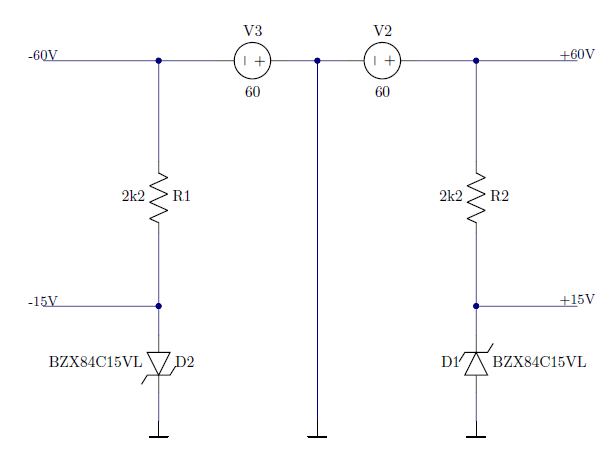
\includegraphics[width=0.7\textwidth]{ImagenesAlimentacion/al.png}
	\caption{Fuente de alimentación}
	\label{fig:alimentacion}
\end{figure}
El diodo seleccionado es uno cuya tensión de zener es de 15V.
Para el cálculo de la resistencia del diodo se tuvo en cuenta que el diodo quede polarizado con una corriente de mantenimiento de 6mA al igual que haya suficiente corriente en la rama para que el par diferencial utilice. Teniendo en cuenta la corriente de polarización del par diferencial se llega  ala conclusión de que la corriente por la resistencia debe ser de 20mA.
\begin{align}
R1=\frac{60-V_z}{20mA}= 2k2\Omega
\end{align}
